\section{Ejercicio 5}


Para este ejercicio se pedía ejecutar y graficar el lote de tareas del ejercicio 2 utilizando el scheduler \emph{Round-Robin} con quantum de 2, 5 y 10, y luego calcular la \textit{latencia}, el \textit{waiting time} y el tiempo total de ejecución de las tareas para cada quantum.

\subsection{Lote Ejecutado Con Quantum 2}

\begin{figure}[!h]
	\begin{center}
		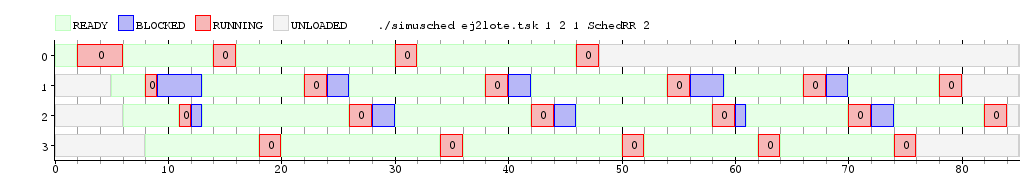
\includegraphics[width=500px]{imagenes/ej5_2.png}
		\caption{Ejecución del lote \emph{ej2lote} con quantum 2.}
		\label{fig:grafico_ej5_2}
	\end{center}
\end{figure}


\subsubsection{Latencia} \label{explicacion_latencia}

Con el gráfico obtenido calculamos la \emph{latencia}. Ésta consiste en el tiempo en que el proceso tarda en comenzar a ejecutarse una vez que el proceso fue cargado en el scheduler.

%LATENCIA
\begin{center}
	\begin{tabular}{|c|c|c|c|c|}
		\hline
		\multicolumn{5}{|c|}{\large{\textbf{Latencia}}} \\
		\hline
		\textbf{Quantum} & \textbf{TaskCPU @0} & \textbf{TaskConsola @5} & \textbf{TaskConsola @6} & \textbf{TaskCPU @8} \\
		\hline
		2 & 2 & 3 & 5 & 10 \\
		\hline
	\end{tabular}
\end{center}


\subsubsection{Waiting Time} \label{explicacion_waiting_time}

Ahora procedemos a calcular el \emph{waiting time} del gráfico obtenido. Éste consiste en el tiempo en que el proceso está en estado de \textit{ready} dentro del scheduler.

%WAITING TIME
\begin{center}
	\begin{tabular}{|c|c|c|c|c|}
		\hline
		\multicolumn{5}{|c|}{\large{\textbf{Waiting Time}}} \\
		\hline
		\textbf{Quantum} & \textbf{TaskCPU @0} & \textbf{TaskConsola @5} & \textbf{TaskConsola @6} & \textbf{TaskCPU @8} \\
		\hline
		2 & 38 & 51 & 59 & 58 \\
		\hline
	\end{tabular}
\end{center}

\subsubsection{Tiempo Total De Ejecución} \label{explicacion_tiempoTDE}

Por último, calculamos el tiempo total de ejecución de un proceso. Éste consiste en calcular el tiempo desde que un proceso es ingresado al scheduler hasta que finaliza.

%TIEMPO TOTAL DE EJECUCION
\begin{center}
	\begin{tabular}{|c|c|c|c|c|}
		\hline
		\multicolumn{5}{|c|}{\large{\textbf{Tiempo Total De Ejecución}}} \\
		\hline
		\textbf{Quantum} & \textbf{TaskCPU @0} & \textbf{TaskConsola @5} & \textbf{TaskConsola @6} & \textbf{TaskCPU @8} \\
		\hline
		2 & 48 & 75 & 78 & 68 \\
		\hline
	\end{tabular}
\end{center}

\newpage

\subsection{Lote Ejecutado Con Quantum 5}

\begin{figure}[!h]
	\begin{center}
		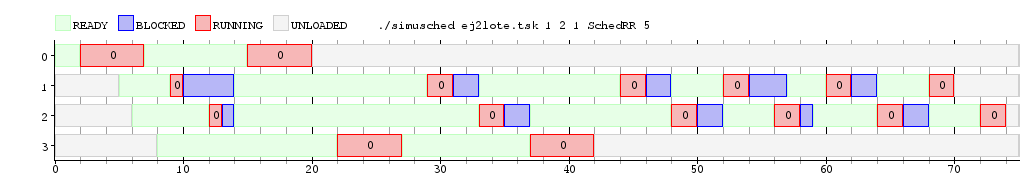
\includegraphics[width=500px]{imagenes/ej5_5.png}
		\caption{Ejecución del lote \emph{ej2lote} con quantum 5.}
		\label{fig:grafico_ej5_5}
	\end{center}
\end{figure}

Con el nuevo gráfico generado calculamos las mismas tres metricas calculadas para el gráfico anterior con un quantum de dos.

\subsubsection{Latencia}

Procedemos a calcular la \emph{latencia}. En la sección \ref{explicacion_latencia} se puede encontrar una breve explicación de la misma.

%LATENCIA
\begin{center}
	\begin{tabular}{|c|c|c|c|c|}
		\hline
		\multicolumn{5}{|c|}{\large{\textbf{Latencia}}} \\
		\hline
		\textbf{Quantum} & \textbf{TaskCPU @0} & \textbf{TaskConsola @5} & \textbf{TaskConsola @6} & \textbf{TaskCPU @8} \\
		\hline
		5 & 2 & 4 & 6 & 14 \\
		\hline
	\end{tabular}
\end{center}

\subsubsection{Waiting Time}

Ahora procedemos a calcular el \emph{waiting time}. En la sección \ref{explicacion_waiting_time} se puede encontrar una breve explicación de esta metrica.

%WAITING TIME
\begin{center}
	\begin{tabular}{|c|c|c|c|c|}
		\hline
		\multicolumn{5}{|c|}{\large{\textbf{Waiting Time}}} \\
		\hline
		\textbf{Quantum} & \textbf{TaskCPU @0} & \textbf{TaskConsola @5} & \textbf{TaskConsola @6} & \textbf{TaskCPU @8} \\
		\hline
		5 & 10 & 39 & 49 & 22 \\
		\hline
	\end{tabular}
\end{center}

\subsubsection{Tiempo Total De Ejecución}

Por último, calculamos el \emph{tiempo total de ejecución} del lote en el scheduler. En la sección \ref{explicacion_tiempoTDE} se puede encontrar una breve explicación de esta métrica.

%TIEMPO TOTAL DE EJECUCION
\begin{center}
	\begin{tabular}{|c|c|c|c|c|}
		\hline
		\multicolumn{5}{|c|}{\large{\textbf{Tiempo Total De Ejecución}}} \\
		\hline
		\textbf{Quantum} & \textbf{TaskCPU @0} & \textbf{TaskConsola @5} & \textbf{TaskConsola @6} & \textbf{TaskCPU @8} \\
		\hline
		5 & 20 & 65 & 68 & 34 \\
		\hline
	\end{tabular}
\end{center}

\subsection{Lote Ejecutado Con Quantum 10}

\begin{figure}[!h]
	\begin{center}
		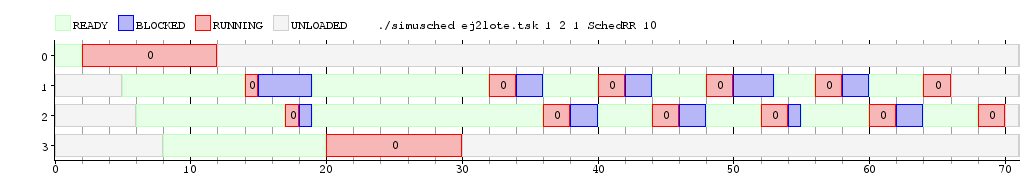
\includegraphics[width=500px]{imagenes/ej5_10.png}
		\caption{Ejecución del lote \emph{ej2lote} con quantum 10.}
		\label{fig:grafico_ej5_10}
	\end{center}
\end{figure}

Con este último gráfico pasamos a realizar las métricas.

\subsubsection{Latencia}

Calculamos la \emph{latencia}. En la sección \ref{explicacion_latencia} se puede encontrar una breve explicación de la misma.

%LATENCIA
\begin{center}
	\begin{tabular}{|c|c|c|c|c|}
		\hline
		\multicolumn{5}{|c|}{\large{\textbf{Latencia}}} \\
		\hline
		\textbf{Quantum} & \textbf{TaskCPU @0} & \textbf{TaskConsola @5} & \textbf{TaskConsola @6} & \textbf{TaskCPU @8} \\
		\hline
		10 & 2 & 9 & 11 & 12 \\
		\hline
	\end{tabular}
\end{center}

\subsubsection{Waiting Time}

Ahora calculamos el \emph{waiting time} sobre el mismo gráfico con un quantum de 10. En la sección \ref{explicacion_waiting_time} se puede encontrar una breve explicación de esta métrica.

%WAITING TIME
\begin{center}
	\begin{tabular}{|c|c|c|c|c|}
		\hline
		\multicolumn{5}{|c|}{\large{\textbf{Waiting Time}}} \\
		\hline
		\textbf{Quantum} & \textbf{TaskCPU @0} & \textbf{TaskConsola @5} & \textbf{TaskConsola @6} & \textbf{TaskCPU @8} \\
		\hline
		10 & 2 & 37 & 45 & 12 \\
		\hline
	\end{tabular}
\end{center}

\subsubsection{Tiempo Total De Ejecución}

Por último, calculamos el \emph{tiempo total de ejecución}. En la sección \ref{explicacion_tiempoTDE} se puede encontrar una breve explicación de la métrica.

%TIEMPO TOTAL DE EJECUCION
\begin{center}
	\begin{tabular}{|c|c|c|c|c|}
		\hline
		\multicolumn{5}{|c|}{\large{\textbf{Tiempo Total De Ejecución}}} \\
		\hline
		\textbf{Quantum} & \textbf{TaskCPU @0} & \textbf{TaskConsola @5} & \textbf{TaskConsola @6} & \textbf{TaskCPU @8} \\
		\hline
		10 & 12 & 61 & 64 & 22 \\
		\hline
	\end{tabular}
\end{center}


\subsection{Análisis De Datos}

Para poder realizar un buen análisis de datos, calculamos el promedio de cada una de las métricas anteriores para cada quantum y así obtener una visión global de éstas.

\subsubsection{Latencia Promedio}

\begin{center}
	\begin{tabular}{|c|c|}
		\hline
		\textbf{Quantum} & \textbf{Latencia Promedio} \\
		\hline
		2 & 5 \\
		\hline
		5 & 6,5 \\
		\hline
		10 & 8,5 \\
		\hline
	\end{tabular}
\end{center}

Se puede en el cuadro como aumenta la \emph{latencia} promedio a medida que el quantum aumenta y esto tiene sentido ya que al tener menos quantum, los procesos son desalojados más rapido y dan lugar a que se ejecuten los demás procesos en la cola.

La diferencia con el scheduler \textbf{FCFS} es muy grande ya que en ese scheduler hasta que no termine el proceso que está en el tope de la cola no pasa al siguiente. La latencia promedio del scheduler \textbf{FCFS} es de $25,5$ (calculada sobre la ejecución del lote con un sólo núcleo), mucho más alta que la de éste scheduler.

\subsubsection{Waiting Time Promedio}

\begin{center}
	\begin{tabular}{|c|c|}
		\hline
		\textbf{Quantum} & \textbf{Waiting Time Promedio} \\
		\hline
		2 & 51,5 \\
		\hline
		5 & 30 \\
		\hline
		10 & 24 \\
		\hline
	\end{tabular}
\end{center}

A diferencia de la \emph{latencia}, se puede apreciar que cuanto mas quantum se le de a los procesos su \emph{waiting time} va a ser menor y esto se debe a que se realizan muchos menos cambios de contexto que resultan costos en tiempo.

\subsubsection{Tiempo De Ejecución Promedio}

\begin{center}
	\begin{tabular}{|c|c|}
		\hline
		\textbf{Quantum} & \textbf{Tiempo De Ejecución Promedio} \\
		\hline
		2 & 67,25 \\
		\hline
		5 & 46,75 \\
		\hline
		10 & 39,75 \\
		\hline
	\end{tabular}
\end{center}

Al igual que el \emph{waiting time} promedio, se puede apreciar una disminución en el \emph{tiempo de ejecución} de los procesos a medida que el quantum aumenta. Esto se debe a que los procesos tienen más tiempo de cpu para realizar calculos y pueden terminar más rápido los que tengan menos llamadas bloqueantes.

Se puede apreciar en los gráficos que, por ejemplo, en el que el lote fue ejecutado con un quantum de dos los procesos ocupan todos un tiempo muy parecido manteniendose así hasta el final, mientras que en el gráfico que fue ejectuado con un quantum de 10 se diferencian mucho los procesos que tienen más uso del cpu de los que realizan muchas llamadas bloqueantes, siendo estos últimos los que continuan ejecutandose mas tiempo.